Now that we have understood the notions of limits and continuity, we can turn to defining the notion of the multivariable derivative.

Let us first recall the notion of the derivative of a single-variable function:


\begin{definition}
    A function $f : D \subset \R \to \R$ is \textbf{differentiable} at a point $x_0 \in D$ if 

    \begin{itemize}
        \item There exists $\delta$ such that $B_\delta(x_0) \subseteq D$
        \item The following limit exists:  $$\lim_{h \to 0} \frac{f(x_0+h) - f(x_0)}{h} = L$$
    \end{itemize}

    If $f$ is differentiable at $x_0$, we say that $L$ is \textbf{the derivative of $f$ at $x_0$}, and we write $$f'(x_0) := L$$
    (sometimes written $\frac{df}{dx}(x_0) = L$)
    \end{definition}

In other words, the derivative depends precisely on the local behavior of $f(x)$ near $x_0$.  That is, we look precisely at the behavior of $f(x)$ in a small neighborhood $B_\varepsilon(x_0)$.

\fixthis{interior point}


The notion of the derivative in single-variable calculus has many interpretations:

\begin{itemize}
    \item The derivative $f'(a)$ tells us the slope of the tangent line to the graph $y=f(x)$ at the point $x=a$.
    \item The derivative $f'(a)$ tells us the instantaneous rate of change of $f(x)$ at the point $x=a$.
    \item The derivative $\frac{d}{dx}$ is an operator, whose input is a differentiable function $f : \R \to \R$, and whose output is a function $f' : \R \to \R$.
    \item The derivative is the linear approximation of $f(x)$ in a small neighborhood $B_\varepsilon(x_0)$.
\end{itemize}

We will see how all of these various notions generalize to the case of multivariable functions.


\section{The Multivariable Derivative}

It takes some thought to come up with the correct definition of the derivative of a multivariable function $f : \R^n \to \R$ at a point $\bm{x_0}$!  

For instance, one might na\"ively define the multivariable derivative as the following limit:
$$f'(\bm{x_0}) \ ``=" \ \lim_{\bm{h} \to \bm{0}} \frac{f(\bm{x_0+h})-f(\bm{x_0})}{||\bm{h}||}$$

However, this definition \textbf{fails} for multiple reasons:

\begin{example}\label{derivfail1}
    Let $f : \R^2 \to \R$ be the function $f(x,y) = x$, and consider the point $\bm{x_0} = (0,0)$.  
    
    We see that $$\lim_{(x,y) \to (0,0) } \frac{f(x,y)-f(0,0)}{||\langle x,y\rangle||}$$
    \textbf{does not exist} by considering the following sequences:

    \begin{itemize}
        \item Along the sequence $\bm{x_n} = \langle \frac{1}{n}, 0 \rangle$, we have that $$\lim_{n\to\infty} \frac{f(\frac{1}{n}, 0)}{||\langle \frac{1}{n}, 0\rangle||} = 1$$
        \item Along the sequence $\bm{y_n} = \langle \frac{1}{n}, 0 \rangle$, we have that $$\lim_{n\to\infty} \frac{f(\frac{-1}{n}, 0)}{||\langle \frac{-1}{n}, 0\rangle||} = -1$$
        \item Along the sequence $\bm{z_n} = \langle 0, \frac{1}{n}\rangle$, we have that $$\lim_{n\to\infty} \frac{f(0, \frac{1}{n})}{||\langle 0, \frac{1}{n}\rangle||} = 0$$
    \end{itemize}
    
\end{example}

Moreover, this definition also fails because it does not correctly generalize the notion of the single variable derivative:

\begin{example}\label{derivfail2}
    Specializing the na\"ive definition to $n=1$, we obtain $\lim_{x \to 0 } \frac{f(x)-f(0)}{|x|}$.

    However, if we consider the function $f: \R \to \R$ defined by $f(x) = |x|$.  We know from single-variable calculus that this function is not differentiable at $x=0$.

    Nevertheless, we see that $$\lim_{x \to 0 } \frac{f(x)-f(0)}{|x|} = 1$$
    
\end{example}

\begin{remark}
    One can correct for the issue in \ref{derivfail2} by instead considering $$\lim_{\bm{h} \to \bm{0}} \frac{|f(\bm{x_0+h})-f(\bm{x_0})|}{||\bm{h}||}$$

    Nevertheless, the issue in \ref{derivfail1} continues to exist for the $f(x,y) = x$ at $(0,0)$ by considering the sequences $\bm{x_n} = \langle \frac{1}{n}, 0 \rangle$ and $\bm{z_n} = \langle 0, \frac{1}{n}\rangle$.
\end{remark}

Thus, we must make a paradigm shift in how we think of the multivariable derivative:


\begin{motivating}
    How should we interpret the multivariable derivative?
\end{motivating}


    The derivative of a single variable function $f(x)$ at a point $x_0$ is the \textbf{approximation} of $f(x)$ by a linear transformation at $x_0$.

\begin{definition}
    A single variable function is \textbf{differentiable at }$x_0$ if there exists a linear transformation $T: \R \to \R$ such that 
    
    $$\lim_{h \to 0} \bigg|\frac{f(x_0+h)-f(x_0)-T(h)}{h}\bigg| = 0$$
    
    Observe that by our characterization of linear transformations $T: \R \to \R$, correspond to scalars $m in \R$ via the correspondence    
    $$T(x) = mx$$  
    We define the derivative of $f$ at $x_0$ to be $m$. That is,    
    $$f'(x_0) := m$$
    \end{definition}

We can generalize this definition as follows:

\begin{definition}
    A multivariable function $f : A \subset R^m \to \R^n$ is \textbf{differentiable at}\define{Multivariable derivative} an interior point $\bm{x_0}$ of $A$  if there exists a linear transformation $T: \R^m \to \R^n$ such that 
    
    $$\lim_{\bm{h} \to \bm{0}} \frac{||f(\bm{x_0+h})-f(\bm{x_0})-T(\bm{h})||}{||\bm{h}||} = 0$$
    
    The \textbf{derivative} of $f$ at $x_0$ is the linear transformation $$Df(\bm{x_0}) := T$$

    By our characterization of linear transformations, $Df(\bm{x_0}) : \R^m \to \R^n$ corresponds to a matrix $[Df(\bm{x_0})] \in M_{n\times m}(\R)$
    \end{definition}

\begin{remark}
    The derivative of a function $f : \R^m \to \R^n$ at a point $x_0$ is the \textbf{approximation} of $f$ by a \textbf{linear transformation} $Df(\bm{x_0})$ at $x_0$.
    \end{remark}

    \begin{proposition}[Uniqueness]
    Suppose $f : A \subset \R^m \to \R^n$ is differentiable at $\bm{x_0}$.
       
    \vspace{1em}
    Then the derivative $Df(\bm{x_0}) : \R^m \to \R^n$ is unique.
    \end{proposition}

    \begin{example}        
The constant map $c: \R^m \to \R^n$ defined by $c(\bm{x}) = \bm{a}$ is differentiable everywhere, and $Dc(\bm{x_0}) = 0$.
    \end{example}

    \begin{example}\label{derivlinearmap}
    A linear map $T: \R^m \to \R^n$ is differentiable everywhere, and $DT(\bm{x_0}) = T$.
    \end{example}

    \begin{proposition}
Suppose that $f, g : A \to \R^n$ are differentiable at $x_0  \in A^\circ$. Then $f+g$ and $\lambda f$ are differentiable at $x_0 \in A^\circ$.
\end{proposition}

    \begin{proposition}[Differentiability implies continuity]
    Suppose $f : A \subset \R^m \to \R^n$ is differentiable at $\bm{x_0}$. 
    
    \vspace{1em}
    Then $f$ is continuous at $\bm{x_0}$.
    \end{proposition}

    \begin{theorem}[The Chain rule]
    Suppose that $g: \R^k \to \R^m$ is differentiable at $x_0 \in \R^k$, and $f : \R^m \to \R^n$ is differentiable at $g(\bm{x_0}) \in \R^m$.  
    
    \vspace{1em}
    
    Then $f \circ g : \R^k \to \R^n$ is differentiable at $x_0 \in \R^k$, and 
    $$D(f \circ g)(\bm{x_0}) = D(f)(g(\bm{x_0})) \circ Dg(\bm{x_0})$$
    
    \end{theorem}


\subsection{The derivative of a vector valued function}

\begin{theorem}
    Let $\bm{r}(t) = \langle x_1(t), \cdots, x_n(t) \rangle$ be a vector-valued function.  
    
    The \textbf{derivative} of $\bm{r}(t) : \R \to \R^n$ at an interior point $\bm{t_0}$ is the linear transformation $T: \R \to \R^n$ given by 
    $$T = 
\begin{bmatrix}
x_1'(t_0) \\
\vdots \\
x_n'(t_0) \\
\end{bmatrix}$$
We sometimes write this derivative as $\bm{r}'(t) : \R \to \R^n$.
\end{theorem}


\begin{theorem}
    A vector-valued function $\bm{r}(t)= \langle x_1(t), \cdots, x_n(t) \rangle$ is differentiable if and only if the functions $x_i(t)$ are differentiable.
     $$\bm{r}'(t) = \langle x_1'(t), \cdots, x_n'(t) \rangle$$
\end{theorem}

    We can think of the derivative $\bm{r}'(t)$ as a tangent vector to the parametric curve of $\bm{r}(t)$.


\begin{definition}
    The \textbf{tangent line} at $\bm{r}(t_0)$ is the line determined by the direction vector $\bm{r}'(t_0)$ and the point $\bm{r}(t_0)$.  That is, the line can be parametrized as 
    $$\bm{L}(t) = \bm{r}(t_0) + t\bm{r}'(t_0)$$
    \end{definition}

\fixthis{picture}

\begin{theorem}[Differentiation Rules]
       Assume that $\bm{r}(t)$ and $\bm{s}(t)$ are differentiable vector-valued functions $\R \to \R^n$..
       
      \begin{enumerate}
        \item $\frac{d}{dt}(\bm{r}(t) + \bm{s}(t)) = \bm{r}'(t) + \bm{s}'(t)$ 
        \item \textbf{Scalar product rule}. For any differentiable scalar-valued function $f(t)$, 
        $$\frac{d}{dt}(f(t)\bm{r}(t)) = f(t)\bm{r}'(t) + f'(t)\bm{r}(t)$$   
        \vspace{-1em}
        \item \textbf{Chain rule}. For any differentiable scalar-valued function $f(t)$, $$\frac{d}{dt}(\bm{r}(f(t))) =  \bm{r}'(f(t))f'(t)$$  
    \end{enumerate}
    \end{theorem}

\begin{theorem}[Dot product rule]
       Assume that $\bm{r}(t)$ and $\bm{s}(t)$ are differentiable vector-valued functions $\R \to \R^n$. Then
       $$\frac{d}{dt}(\bm{r}(t) \cdot \bm{s}(t)) = \bm{r}'(t)\cdot\bm{s}(t) + \bm{r}(t)\cdot\bm{s}'(t)$$ 
    \end{theorem}
    
       
    \begin{theorem}[Cross product rule]
       Assume that $\bm{r}(t)$ and $\bm{s}(t)$ are differentiable vector-valued functions $\R \to \R^3$. Then 
       $$\frac{d}{dt}(\bm{r}(t) \times \bm{s}(t)) = \bm{r}'(t)\times \bm{s}(t) + \bm{r}(t)\times \bm{s}'(t)$$
    \end{theorem}

\subsection{The derivative of multivariable functions}

\begin{motivating}
    How should we think of the derivative of a multivariable function $f: \R^n \to \R$?
    \end{motivating}

Given a function $g: \R^n \to \R$, we can graph it as a surface $x_{n+1} = g(x_1, \cdots, x_n)$ in $\R^{n+1}$, which has points $$(x_1,\cdots, x_n, g(x_1, \cdots, x_n))$$
    
    
    If $T$ is the derivative of a function $f: \R^n \to \R$, then $T : \R^n \to \R$ is a linear map, which corresponds to a $n \times 1$ matrix.
    \begin{equation*}
T(x_1, \cdots, x_n) = A\begin{bmatrix}
x_1 \\
\vdots\\
x_n
\end{bmatrix}
=
\begin{bmatrix}
a_1 & \cdots & a_n
\end{bmatrix}\begin{bmatrix}
x_1 \\
\vdots\\
x_n
\end{bmatrix}
= \sum_i^n a_ix_i
\end{equation*}

\begin{proposition}
The graph of $T : \R^n \to \R$ is the hyperplane $x_{n+1} = \sum_i^n a_ix_i$.
\end{proposition}

\begin{definition}
    The \textbf{$i$-th partial derivative} $D_if$ of a multivariable function $f : A \subset \R^m \to \R$ for $\bm{x_0} \in A^\circ$ is defined as the limit
    $$D_if(\bm{x_0}) =  \lim_{t \to 0} \frac{f(\bm{x_0}+t\bm{e_i})-f(\bm{x_0})}{t}, \qquad i = 1, \cdots, n$$
    if it exists.
    
    \end{definition}

    \begin{example}
        Let $f: \R^2 \to \R$ be defined by $f(x,y) = xe^{xy}$.  Then the partial derivatives of $f$ are
        $$\frac{\partial f}{\partial x} = xye^{xy} + e^{xy} \qquad \frac{\partial f}{\partial y} = x^2e^{xy}$$
    \end{example}
    

\begin{proposition}
    Given a graph of $z = f(x_1, \cdots, x_n)$, the tangent (hyperplane) in $\R^{n+1}$ is spanned by vectors of the form $\bm{e_i} + \frac{\partial f}{\partial x_i}\bm{e_{n+1}}$
    \end{proposition}
    
    \fixthis{picture}
    
    \begin{proposition}
    We can take the normal vector of the tangent hyperplane in $\R^{n+1}$ to the graph of a multivariable function $f : \R^n \to \R$ to be 
    $$\bm{n} = \sum_{i}^n \left(\frac{\partial f}{\partial x_i}\bm{e_i}\right) -\bm{e_{n+1}} = \left\langle \frac{\partial f}{\partial x_1}, \cdots, \frac{\partial f}{\partial x_n}, -1\right\rangle $$
    \end{proposition}

    \begin{theorem}
    Let $\bm{a} = \langle a_1, \cdots, a_n \rangle \in \R^n$.  The equation of the tangent hyperplane in $\R^{n+1}$ to the graph of a multivariable function $f(\bm{a}) : \R^n \to \R$ at a point $$\bm{\overline{a}} = (a_1, \cdots, a_n, f(\bm{a}))$$ is given by 
    
    %\pause
    
    $$\left\langle \frac{\partial f}{\partial x_1}, \cdots, \frac{\partial f}{\partial x_n}, -1 \right\rangle \cdot (\bm{x} - \bm{\overline{a}}) = 0$$

    Equivalently, $$x_{n+1} = f(\bm{a}) + \begin{bmatrix}
D_1f(\bm{a}) & D_2f(\bm{a}) & \cdots & D_nf(\bm{a})
\end{bmatrix} (\bm{x} - \bm{a}) $$
    \end{theorem}

 We can use the multivariable derivative to approximate multivariable functions!

 \begin{theorem}[Linear approximation]
    
    If $f : A \subset \R^m \to \R$ is \underline{differentiable} at a point $\bm{a} = (a_1, \cdots, a_n)$, and $\bm{x}= (x_1, \cdots, x_n)$ is close to $\bm{a}$, then 
    \begin{align*}
     f(\bm{x}) &\approx f(\bm{a}) + \begin{bmatrix}
D_1f(\bm{a}) & D_2f(\bm{a}) & \cdots & D_nf(\bm{a})
\end{bmatrix} (\bm{x} - \bm{a}) \\
    &= f(\bm{a}) + \sum_{i}^n \left(\frac{\partial f}{\partial x_i}(\bm{a})\right)(x_i - a_i)   
    \end{align*}
    
    \end{theorem}

Equivalently, one can say that the change in $f$ near $\bm{a}$ can be approximated by the partial derivatives and the change in $x_i$.
    
    
    $$\Delta f \approx \sum_{i}^n \left(\frac{\partial f}{\partial x_i}(\bm{a})\right)\Delta x_i$$

\subsection{The multivariable derivative in coordinates}

\begin{motivating}
    How do we calculate the linear transformation $Df(\bm{x_0})$ for general multivariable functions $f : A \subset \R^m \to \R^n$?
    \end{motivating}


\begin{definition}
    Let $f : A \subset \R^m \to \R^n$ be a multivariable function defined by $f_i  : A \subset \R^m \to \R$:
    \begin{equation*}
        f(\bm{x}) = \begin{bmatrix}
f^1(\bm{x}) \\
\vdots \\
f^n(\bm{x})
\end{bmatrix}
    \end{equation*}
    
    The \textbf{Jacobian matrix} of $f$ at $\bm{x_0}$ is 
    
    \begin{equation*}
        [J_f(\bm{x_0})] = \begin{bmatrix}
D_1f^1(\bm{x_0}) & D_2f^1(\bm{x_0}) & \cdots & D_mf^1(\bm{x_0}) \\
D_1f^2(\bm{x_0}) & D_2f^2(\bm{x_0}) & \cdots & D_mf^2(\bm{x_0}) \\
\vdots & \vdots & \vdots & \vdots\\
D_1f^n(\bm{x_0}) & D_2f^n(\bm{x_0}) & \cdots & D_mf^n\bm{x_0}) 
\end{bmatrix}
    \end{equation*}
    
    if the partial derivatives exist.
    
    \end{definition}

\begin{theorem}[The derivative in coordinates]
    Let  $f : A \subset \R^m \to \R^n$ be a multivariable function.  If $f$ is \textbf{differentiable at} $\bm{x_0}$, then all the partial derivatives $D_if^j\bm{x_0})$ exist, and the standard matrix of $Df(\bm{x_0})$ is $[J_f(\bm{x_0})]$.  That is,
    $$Df(\bm{x_0})(\bm{h}) = [J_f(\bm{x_0})]\bm{h}$$
    
    \end{theorem}

    \begin{example}
    Consider the transformation from polar coordinates to rectangular coordinates, which is the function $f(r,\theta) : (0, \infty) \times [0, 2\pi) \subset \R^2 \to \R^2$ given by $$f(r, \theta) = \langle r\cos(\theta), r\sin(\theta) \rangle$$

    Then the Jacobian of $f$ is the matrix

\begin{equation*}
        [J_f(r, \theta)] = \begin{bmatrix}
\cos(\theta), -r\sin(\theta) \\
\sin(\theta), r\cos(\theta)  
\end{bmatrix}
    \end{equation*}
    
    \end{example}
    
    
    \begin{remark}
    The converse does not hold - there exists functions $f$ such that all the partial derivatives exist at some point $\bm{x_0}$, but $f$ is \underline{not} differentiable at $\bm{x_0}$.
    \end{remark}    

\begin{example}
    Consider the function $f(x,y) = \left\{
		\begin{array}{ll}
			\frac{xy}{x^2 + y^2} & \text{ if } (x,y) \neq (0,0) \\
			0 & \text{ otherwise } 
		\end{array}
		\right.$

  Then the partial derivatives of $f$ exist at $(0,0)$, but $f$ is not continuous at $(0,0)$!
\end{example}

\fixthis{picture}

    \begin{example}
    Consider the function  $f(x,y) = \left\{
		\begin{array}{ll}
			\frac{2xy(x+y)}{x^2+y^2} & \text{ if } (x,y) \neq (0,0) \\
			0 & \text{ otherwise } 
		\end{array}
		\right.$

    Then the partial derivatives exist at $(0,0)$, but $f$ is not differentiable at $(0,0)$.  You will prove this in the exercises below.
\end{example}

\fixthis{picture}

However, if we strengthen the hypotheses, then we do have the following result:
    
    \begin{theorem}
    Let  $f : A \subset \R^m \to \R^n$ be a multivariable function.  If all the partial derivatives $D_if^j\bm{x_0})$ \underline{exist and are continuous in some open ball} $B_\varepsilon(\bm{x_0})$, then $f$ is differentiable at $\bm{x_0}$.
    \end{theorem}

\subsection{The chain rule}

Let us now revisit the previous theorems, now that we can compute general multivariable derivatives!

\begin{theorem}[The Chain rule]
    Let $f : \R^n \to \R^m$, and let $g: \R^m \to \R^k$ be multivariable functions such that $f$ is differentiable at $\bm{x_0} \in \R^n$, and $g$ is differentiable at $f(\bm{x_0}) \in \R^m$.
    
    \vspace{1em}
    Then $g \circ f : \R^n \to \R^k$ is differentiable at $\bm{x_0} \in \R^n$, and 
    
    $$D(g \circ f)(\bm{x_0}) = Dg(f(\bm{x_0})) \circ Df(\bm{x_0})$$
    
    \end{theorem}

We can prove this using the definition of derivative.

However, since we know that the derivative can be computed in terms of the Jacobian, we equivalently have

    \begin{theorem}[The Chain rule in coordinates]
        Suppose that $f : \R^n \to \R^m$ is differentiable at $\bm{x_0} \in \R^n$, and $g: \R^m \to \R^k$ is differentiable at $f(\bm{x_0}) \in \R^m$.   Then
    $$[J_{g\circ f}(\bm{x_0})] =\left[J_g(f(\bm{x_0}))\right][J_f(\bm{x_0})]$$
    \end{theorem}

We can spell this out in terms of coordinates:

\begin{example}
    Suppose that $f : \R^n \to \R^m$ is differentiable at $\bm{x_0} \in \R^n$, and $g: \R^m \to \R^k$ is differentiable at $f(\bm{x_0}) \in \R^m$. Then
\begin{multline}
        \begin{bmatrix}
D_1(g \circ f)^1(\bm{x_0}) & \cdots & D_n(g \circ f)^1(\bm{x_0}) \\
\vdots & \vdots & \vdots\\
D_1(g \circ f)^k(\bm{x_0}) & \cdots & D_n(g \circ f)^k(\bm{x_0}) \\
\end{bmatrix} = \\
\begin{bmatrix}
D_1g^1(f(\bm{x_0})) & \cdots & D_mg^1(f(\bm{x_0})) \\
\vdots & \vdots & \vdots\\
D_1g^k(f(\bm{x_0}))  & \cdots & D_mg^k(f(\bm{x_0})) 
\end{bmatrix}
\begin{bmatrix}
D_1f^1(\bm{x_0}) & \cdots & D_nf^1(\bm{x_0}) \\
\vdots & \vdots & \vdots\\
D_1f^m(\bm{x_0})  & \cdots & D_nf^m(\bm{x_0}) 
\end{bmatrix}
\end{multline}
    \end{example}
    
\begin{motivating}
    How can we compute $D(g \circ f)(\bm{x_0})$?  Equivalently, what are the entries of the matrix $[J_{g\circ f}(\bm{x_0})]$?
\end{motivating}

To answer this question, let us look at the chain rule for a special case: composites of the form $\R^n \to \R^m \to \R$

\begin{example}
    Suppose that $f : \R^n \to \R^m$ is differentiable at $\bm{x_0} \in \R^n$, and $g: \R^m \to \R$ is differentiable at $f(\bm{x_0}) \in \R^m$. Then
    \begin{multline}
        \begin{bmatrix}
D_1(g \circ f)(\bm{x_0}) & \cdots & D_n(g \circ f)(\bm{x_0}) 
\end{bmatrix} = \\
\begin{bmatrix}
D_1g(f(\bm{x_0})) & \cdots & D_mg(f(\bm{x_0})) 
\end{bmatrix}
\begin{bmatrix}
D_1f^1(\bm{x_0}) & \cdots & D_nf^1(\bm{x_0}) \\
\vdots & \vdots & \vdots\\
D_1f^m(\bm{x_0})  & \cdots & D_nf^m(\bm{x_0}) 
\end{bmatrix}
    \end{multline}
    Therefore,
    $$\D_i(g \circ f) = \sum_k  D_i f^k \ D_k g$$
    \end{example}

\begin{corollary}
    Suppose that $f : \R^n \to \R^m$ is differentiable at $\bm{x_0} \in \R^n$, and $g: \R^m \to \R$ is differentiable at $f(\bm{x_0}) \in \R^m$. Then
$$\left[J_{g\circ f}(\bm{x_0})\right] = \left[D_i(g \circ f)^j\right] = \left[\sum_k  D_i f^k \ D_k g^j\right]$$
\end{corollary} 

\begin{example}
    Let $f(x,y,z) = xy + z$.  Calculate $\frac{\partial f}{\partial s}$, where $x = s^2$, $y = st$, $z = t^2$.
\end{example}


Let us now turn to another specific case of the chain rule:  

\begin{proposition}[Chain rule for paths]
    Let $f(x_1, \cdots x_n) : \R^n \to \R$ be a differentiable function, and let $\bm{r}(t) = \langle x_1(t), \cdots, x_n(t) \rangle : \R \to \R^n$ be a vector-valued function.  Then $f(\bm{r}(t)) : \R \to \R$ is a single variable function, and 
    \begin{align*}
        \frac{d}{dt}f(\bm{r}(t_0)) &= \begin{bmatrix}
\frac{\partial f}{\partial x_1}(\bm{r}(t_0)) & \cdots & \frac{\partial f}{\partial x_n}(\bm{r}(t_0))
\end{bmatrix} \begin{bmatrix}
x_1'(t_0) \\
\vdots \\
x_n'(t_0) \\
\end{bmatrix} \\
&= \sum_{i=1}^n
\left(\frac{\partial f}{\partial x_i}(\bm{r}(t_0)) \right) x_i'(t_0)
    \end{align*}
    \end{proposition}


This measures the rate of change of $f$ along the path $\bm{r}(t)$.

\fixthis{PICTURE}



\begin{example}
    Consider the linear path through $\bm{x_0} \in \R^n$ in the direction of a vector $\bm{v}$, say $$\bm{r}(t) = \bm{x_0} + t\bm{v}$$  Observe that the chain rule depends on the magnitude of $\bm{v}$

\end{example}

Let us make a definition that is independent of $||\bm{V}||$

\begin{definition}
    If $\bm{u} = \langle u_1, \cdots, u_n \rangle$ is a unit vector in $\R^n$, then the \textbf{directional derivative}\define{directional derivative}
    in the direction of $\bm{u}$ at the point $\bm{x_0} \in \R^n$ is defined as
    $$D_{\bm{u}} f(\bm{x_0}) = u_1\frac{\partial f}{\partial x_1}(\bm{x_0}) + \cdots + u_n\frac{\partial f}{\partial x_n}(\bm{x_0})$$
    \end{definition}

The directional derivative measures the rate of change of $f$ in the direction of $\bm{u}$.  That is, $$D_{\bm{u}} f(\bm{x_0}) = \frac{d}{dt}f(\bm{r}(0))$$ for $\bm{r}(t) = \bm{x_0} + t\bm{u}$.

\fixthis{PICTURE}

\begin{example}
    
\end{example}



\subsection{The gradient}


\begin{definition}
    If $f(x_1,\cdots,x_n)$ is a function of $n$ variables, then the \textbf{gradient} of $f$ is the vector-valued function 
    $$\nabla f = \langle \frac{\partial f}{\partial x_1} , \cdots, \frac{\partial f}{\partial x_n} \rangle$$
    That is, $$\nabla f = [Df(\bm{x_0})]^\intercal$$
    where $[A]^\intercal$ indicates the transpose matrix (see definition \ref{transpose}).
    \end{definition}


    
    \begin{proposition}
    The chain rule for paths can be rewritten as
    $$\frac{d}{dt}f(\bm{r}(t_0))= \nabla f(\bm{r}(t_0)) \cdot \bm{r}'(t_0)$$
    
    \end{proposition}

 \begin{corollary}
     If $\bm{u} \in \R^n$ is a unit vector, then the directional derivative
    in the direction of $\bm{u}$ at the point $\bm{P} \in \R^n$ can be computed as
    $$D_{\bm{u}} f(\bm{P}) = \nabla f(\bm{P}) \cdot \bm{u}$$
 \end{corollary}
        
This helps us geometrically interpret the gradient:

\begin{proposition}
    The directional derivative $D_{\bm{u}} f$ is \textbf{maximized} when $\theta = 0$, so when $\bm{u} = \bm{e}_{\nabla f}$.  The maximum value of $D_{\bm{u}} f$ is $||\nabla f||$.

    
    The directional derivative $D_{\bm{u}} f$ is \textbf{minimized} when $\theta = \pi$, so when $\bm{u} = -\bm{e}_{\nabla f}$.  The minimum value of $D_{\bm{u}} f$ is $-||\nabla f||$.
    \end{proposition}
    
    \begin{example}
        Thinking of $z$ as the height of $z = f(x,y)$, the gradient $\nabla f$ points in the direction of \textbf{steepest ascent}.
    
    \vspace{1em}
    
    The opposite of the gradient, $-\nabla f$, points in the direction of \textbf{steepest descent}.
    \end{example}
    
    Furthermore, if $\bm{r}(t)$ parameterizes a level curve $f(x_1, \cdots, x_n) =k$, recall that means that for all $t$, $$f(\bm{r}(t)) = k$$
    
    
    \begin{proposition}
    The gradient $\nabla f$ is \textbf{orthogonal} to the (tangent lines of) the level curves.
    \end{proposition}

\fixthis{PICTURE}






\begin{corollary}
    Let $f(x_1,\cdots,x_n) : \R^n \to \R$ be a differentiable function at a point $\bm{a} = (a_1,\cdots, a_n)$.  Moreover, suppose that $f(a_1,\cdots,a_n) = k$.  
    
    Then $\nabla f = \bm{0}$, or $\nabla f$ is \textbf{orthogonal} to the surface $$f(x_1,\cdots,x_n) = k$$
    \end{corollary}




\begin{corollary}
    The \textbf{tangent hyperplane} to the surface $f(x_1,\cdots,x_n) = k$ in $\R^n$ at the point $\bm{a} = (a_1,\cdots, a_n)$ is given by 
    $$\nabla f(\bm{a}) \cdot (\bm{x - a}) = 0$$
    \end{corollary}

\begin{motivating}
    How does this relate to previous notions of tangent hyperplane?
\end{motivating}
        
    \begin{theorem}
    The graph of a multivariable function $g(x_1, \cdots, x_n) : \R^n \to \R$ can be described as $$x_{n+1} = g(x_1, \cdots, x_n)$$ in $\R^{n+1}$.  The equation of the tangent hyperplane in $\R^{n+1}$ at a point $$\bm{\overline{a}} = (a_1, \cdots, a_n, g(a_1, \cdots, a_n))$$ is given by 
    
    
    $$\left\langle \frac{\partial g}{\partial x_1}, \cdots, \frac{\partial g}{\partial x_n}, -1 \right\rangle \cdot (\bm{\overline{x}} - \bm{\overline{a}}) = 0$$
    \end{theorem}

    Observe that if we set $f(x_1, \cdots, x_{n+1}) = g(x_1, \cdots, x_n) - x_{n+1}$, then $$\nabla f = \left\langle \frac{\partial g}{\partial x_1}, \cdots, \frac{\partial g}{\partial x_n}, -1 \right\rangle$$

\subsection{Exercises}



\begin{problem}{notderivative1}


    Find a function $f(x) : \R \to \R$ that shows that defining the derivative of a multivariable function as 
    $$f'(\bm{x_0}) = \lim_{\bm{h} \to \bm{0}} \frac{f(\bm{x_0+h})-f(\bm{x_0})}{||\bm{h}||}$$ \textbf{does not} generalize the single variable derivative.


    
\end{problem}

\begin{problem}{notderivative2}

    Consider the function $f(x,y) = x$.  Show that  $$\lim_{\bm{h} \to \bm{0}} \frac{f(\bm{x_0+h})-f(\bm{x_0})}{||\bm{h}||}$$ does not exist at $(0,0)$.  (Hence, this is also not a good definition of the multivariable derivative).
    
\end{problem}


\begin{problem}{approx1}
    Use linear approximation to approximate $\frac{8.01}{\sqrt{(1.99)(2.01)}}$.
\end{problem}

\begin{problem}{approx2}
    Use linear approximation to approximate $(2.92)^2\sqrt{4.08}$.
\end{problem}

\begin{problem}{partialnotcontinuous}
    Consider the function $f(x,y) = \left\{
		\begin{array}{ll}
			\frac{xy}{x^2 + y^2} & \text{ if } (x,y) \neq (0,0) \\
			0 & \text{ otherwise } 
		\end{array}
		\right.$  Use the limit definition of the partial derivative to compute $f_x(0,0)$ and $f_y(0,0)$.
\end{problem}

\begin{problem}{partialderiv1}
    Consider the function $f(x,y) = \left\{
		\begin{array}{ll}
			\frac{x^3}{x^2 + y^2} & \text{ if } (x,y) \neq (0,0) \\
			0 & \text{ otherwise } 
		\end{array}
		\right.$
		
		Use the limit definition of the partial derivative to compute $f_x(0,0)$ and $f_y(0,0)$.
\end{problem}

\begin{problem}{partialderiv2}
    Let $f(u,v) = \tan(uv^3)$.  Find the partial derivatives $f_u(u,v)$ and $f_v(u,v)$.
\end{problem}


\begin{problem}{chainrule1}
    Let $f(x,y,z) = xy + z$.  Calculate $\frac{\partial f}{\partial t}$, where $x = s^2$, $y = st$, $z = t^2$.
\end{problem}

\begin{problem}{chainrule2}
    Let $f(x,y) = \tan(xy^2)$, and consider the path $\bm{r}(t) = \langle t, e^t \rangle$.  Compute $\frac{d}{dt}f(\bm{r}(t))$ at the point $(2,e^2)$.
\end{problem}

\begin{problem}{gradient1}
    Calculate the gradient of $g(x,y,z) = x\ln(y+z)$.
\end{problem}


\begin{problem}{gradient2}
    Find the maximum rate of change of $f(x,y) = e^{xy-y^2}$at the point $(1,1)$.
\end{problem}

\begin{problem}{directionalderiv01}
    Let $f(x,y) = e^{xy-y^2}$. Compute the directional derivative in the direction of $\bm{u} = \langle 5, 12 \rangle$ at the point $P = (1,1)$.
\end{problem}

\begin{problem}{directionalderiv1}
    Find the directional derivative of $g(x,y,z) = xy+z^2$ at the point $P = (3,2,-1)$, in the direction pointing to the origin.
\end{problem}

\begin{problem}{directionalderiv2}
    Find the directional derivative of $g(x,y,z) = x\ln(y+z)$ in the direction of the vector $\bm{v} = \langle 2, -1, 1 \rangle$ at the point $P = (2,e,e)$.
\end{problem}


\begin{problem}{tangentplane1}
    Find an equation of the plane tangent to the graph of $f(x,y) = xy^3 + x^2$ at the point $(2,-2,-12)$
\end{problem}

\section{Optimizing Multivariable functions}

Recall that in single-variable calculus, the derivative is also useful in optimising single-variable functions.  That is, finding local maxima and minima, as well as global maxima and minima.  

\begin{definition}
    A function $f: \R \to \R$ has a \textbf{local maximum} at $P \in \R$ if there exists some $r>0$ such that
    $$f(P) \geq f(Q)$$
    for all points $Q \in B_r(P)$.
    \end{definition}

    \begin{definition}
    A function $f: \R \to \R$ has a \textbf{local minimum} at $P \in \R$ if there exists some $r>0$ such that
    $$f(P) \leq f(Q)$$
    for all points $Q \in B_r(P)$.
    \end{definition}

\begin{definition}
    A function $f: D \subset \R \to \R$ has a \textbf{global maximum on $D$} at $P \in \R$ if
    $$f(P) \geq f(Q)$$
    for all points $Q \in D$.
    \end{definition}

    \begin{definition}
    A function $f: D \subset \R \to \R$ has a \textbf{global minimum on $D$} at $P \in \R$ if 
    $$f(P) \leq f(Q)$$
    for all points $Q \in D$.
    \end{definition}

\begin{motivating}
    How can we find and classify local maxima and minima?
\end{motivating}

\begin{definition}
        A point $P \in \R$ in the domain of $f(x)$ is a \textbf{critical point} if
        
        \begin{enumerate}
            \item $f'(P) = 0$, OR
            \item $f'(P)$ does not exist.
        \end{enumerate}
        
    \end{definition}

    \begin{theorem}[The single-variable first derivative test]
        If $f(x)$ has a local maximum or minimum at $P$, then $P$ is a critical point of $f(x)$.
    \end{theorem}

    We can classify the critical points of $f(x)$ using the single-variable second derivative test (theorem \ref{single2ndderiv}).

    We can also find global maxima and minima of $f(x)$ on an interval $D = [a,b]$:

    \begin{theorem}
    The global maxima and minima of $f(x)$ on $[a,b]$ either occur at the critical points of $f$ in $[a,b]$, or on the boundary of $[a,b]$.
    \end{theorem}

    To classify the global maxima and minima, we simply evaluate the function at these critical points.

    In the following sections, we will see how to generalize these ideas to multivariable calculus:

\subsection{Local optimization}

First, let us define the notion of a local extremum for a multivariable function $f: \R^n \to \R$:

\begin{definition}
    A function $f: \R^n \to \R$ has a \textbf{local maximum} at $\bm{P} \in \R^n$ if there exists some $r>0$ such that
    $$f(\bm{P}) \geq f(\bm{Q})$$
    for all points $\bm{Q} \in B_r(\bm{P})$.
    \end{definition}

    \begin{definition}
    A function $f: \R^n \to \R$ has a \textbf{local minimum} at $\bm{P} \in \R^n$ if there exists some $r>0$ such that
    $$f(\bm{P}) \leq f(\bm{Q})$$
    for all points $\bm{Q} \in B_r(\bm{P})$.
    \end{definition}

\fixthis{Note: local extrema only make sense for functions $f: \R^n \to \R$.}

\begin{definition}
    A function $f : A \subset \R^n \to \R$ has a \textbf{global maximum} at $\bm{x_0} \in A$ if
    $$f(\bm{x_0}) \geq f(\bm{x})$$ 
    for all $\bm{x} \in A$.
    \end{definition}
    
    \begin{definition}
    A function $f : A \subset \R^n \to \R$ has a \textbf{global minimum} at $\bm{x_0} \in A$ if
    $$f(\bm{x_0}) \leq f(\bm{x})$$ 
    for all $\bm{x} \in A$.
    \end{definition}

\begin{remark}
    Observe that \textbf{local} maxima/minima are not necessarily \textbf{global} maxima/minima.
    \end{remark}
    
    \begin{center}
        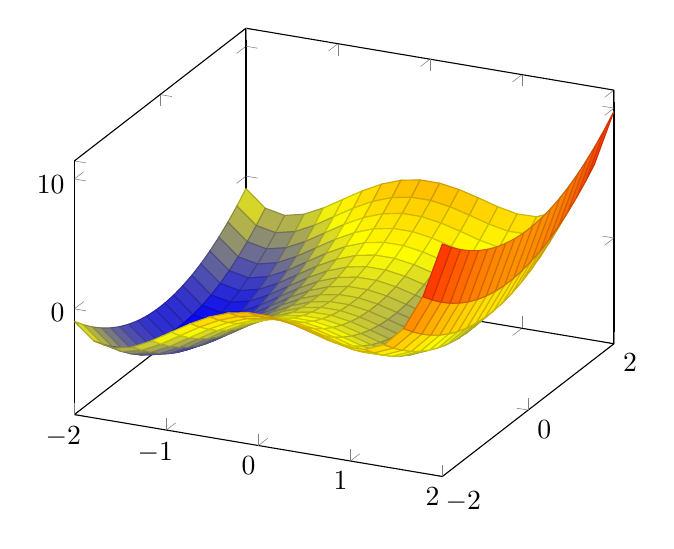
\begin{tikzpicture}
\begin{axis}
 
\addplot3 [
    domain=-2:2,
    domain y = -2:2,
    samples = 20,
    samples y = 20,
    surf] {.9*x^4  + .67*x^3 - 3*x^2 + 2 + y^2 - 4};
 
\end{axis}
 
\end{tikzpicture}
    \end{center}


\begin{motivating}
    What is the multivariable analogue of the first derivative test?
\end{motivating}

\begin{remark}
        Observe that if $\bm{P} \in \R^n$ is a local maxima or minima of $f: \R^n \to \R$, and if $f$ is differentiable at $\bm{P}$, then $Df(\bm{P})$ is the zero linear transformation (equivalently, $\nabla f = \bm{0}$).

        That is, the tangent plane at $\bm{P}$ is parallel to the plane $x_{n+1} = 0$.
    \end{remark}

\begin{definition}
        A point $\bm{P} \in \R^n$ is said to be a \textbf{critical point} of a function $f: \R^n \to \R$ if either

        \begin{enumerate}
            \item $Df(\bm{P}) = 0$, OR
            \item $Df(\bm{P})$ does not exist.
        \end{enumerate}
      
    \end{definition}

\begin{proposition}
     Equivalently, $\bm{P}$ is a critical point of $f: \R^n \to \R$ if
    \begin{enumerate}
            \item $\nabla f(\bm{P}) = \bm{0}$, OR
            \item $\nabla f(\bm{P})$ does not exist.
        \end{enumerate}
\end{proposition}


\begin{theorem}[The multivariable first derivative test]
        If $f: \R^n \to \R$ has a local maximum or minimum at $\bm{P}$, then $\bm{P}$ is a critical point of $f$.
    \end{theorem}


    \begin{remark}
        The converse of the first derivative test does not hold:
        
        If $\bm{P}$ is a critical point of $f$, then $\bm{P}$ is not necessarily a local maximum or minimum.
    \end{remark}

    \begin{example}
        Consider the function $f(x,y) = x^2-y^2$.  Observe that $(0,0)$ is a critical point, but it is neither a local maximum or a minimum.

    \begin{center}
        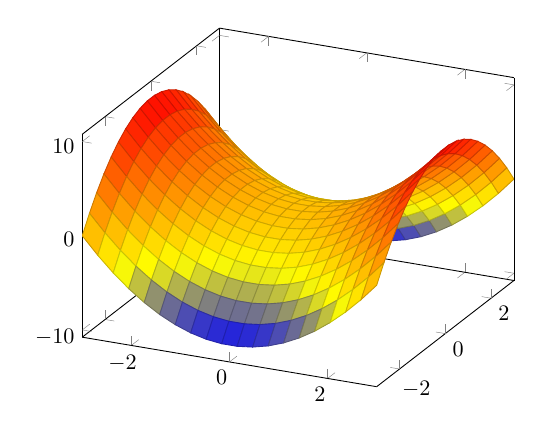
\begin{tikzpicture}[scale=0.8]
 
\begin{axis}
 
\addplot3 [
    domain=-3:3,
    domain y = -3:3,
    samples = 20,
    samples y = 20,
    surf] {x^2 - y^2};
 
\end{axis}
 
\end{tikzpicture}
    \end{center}


    \end{example}

\subsubsection{Classifying local extrema}

\begin{motivating}
    How can we algebraically classify the behavior of critical points?
\end{motivating}

Recall that in single-variable calculus, we can do so using the \textbf{second derivative test}:

\begin{theorem}[The single-variable second derivative test]\label{single2ndderiv}

Let $f : \R \to \R$ be a single variable function.

\begin{enumerate}
    \item If $f'(P) = 0$ and $f''(P) > 0$, then there is a \textbf{local minimum} at $x=P$. 
    \item If $f'(P) = 0$ and $f''(P) < 0$, then there is a \textbf{local maximum} at $x=P$. 
    \item If $f'(P) = 0$ and $f''(P) = 0$, then the test is \textbf{inconclusive}.
\end{enumerate}

If $f''(P)$ does not exist, then the test is \textbf{inconclusive}.

\end{theorem}

\begin{motivating}
    What is the multivariable analogue of the second derivative test?
\end{motivating}

First, we need to figure out what we mean by the second derivative of a multivariable function.

Recall from example \ref{derivlinearmap} that the derivative of a linear transformation $T$ is $T$ itself. That is, 
$$DT(\bm{x_0}) = T$$
Thus, we cannot na\"ively define the second derifative of $f$ as $D(Df(\bm{x_0})$.

\begin{remark}
    We have defined the derivative $Df(\bm{x_0})$ to be the linear approximation of $f$ \textnormal{at a point} $\bm{x_0} \in \R^n$.
    
    This is analogous to finding the slope of the tangent line of a single variable function \textnormal{at a point} $x \in \R$.
    
    \end{remark}

Therefore, we wish to find the derivative of $Df$, not of $Df(\bm{x_0})$, where 
$$Df : \R^n \to M_{1\times n}(\R)$$

However, observe that we have only defined derivatives of functions $f : \R^m \to \R^n$.  We have not defined the derivative of a function that outputs matrices!  However, since we know that $$M_{1\times n}(\R) \cong \R^n$$ via the transpose map $(-)^\intercal$ 
$$M \mapsto M^\intercal$$

We can then consider the map $$(Df)^\intercal : \R^n \cong M_{1\times n}(\R) \to \R^n$$
which sends a vector 
$$\bm{x_0} \mapsto \begin{bmatrix}
D_1f(\bm{x_0}) \\
\vdots \\
D_nf(\bm{x_0})
\end{bmatrix}$$

Observe that $$(Df)^\intercal(\bm{x_0}) =  \nabla f(\bm{x_0})$$  
Thus, we can make the following definition:

\begin{definition}
A multivariable function $f: \R^n \to \R$ is \textbf{twice-differentiable} if $f : \R^n \to \R$ and $\nabla f : \R^n \to \R^n$ are both differentiable.

\vspace{1em}

If $f: \R^n \to \R$ is twice-differentiable, then the \textbf{second derivative of} $f$ \textbf{at} $\bm{x_0}$ is defined as 
$$D^2f(\bm{x_0}) := D(\nabla f)(\bm{x_0})$$
\end{definition}

\begin{definition}
Let $f: \R^n \to \R$ be a twice-differentiable function. Then the standard matrix of $D^2f(\bm{x_0})$ is called the \textbf{Hessian matrix}, 
$$\left[H_f(\bm{x_0})\right]$$
\end{definition}

\begin{proposition}
    The \textbf{Hessian matrix} of $f:\R^n \to \R$ at $\bm{x_0}$ is 
    
    \begin{equation*}
        [H_f(\bm{x_0})] = \begin{bmatrix}
D_1D_1f(\bm{x_0}) & D_2D_1f(\bm{x_0}) & \cdots & D_nD_1f(\bm{x_0}) \\
D_1D_2f(\bm{x_0}) & D_2D_2f(\bm{x_0}) & \cdots & D_nD_2f(\bm{x_0}) \\
\vdots & \vdots & \vdots & \vdots\\
D_1D_nf(\bm{x_0}) & D_2D_nf(\bm{x_0}) & \cdots & D_nD_nf(\bm{x_0}) 
\end{bmatrix}
    \end{equation*}
\end{proposition}

In other words, the Hessian matrix is the $n \times n$ matrix of all second-order partial derivatives of $f$,
    $$f_{x_jx_i} = D_iD_j f = \frac{\partial}{\partial x_i}\left(\frac{\partial f}{\partial x_j}\right)$$


\begin{example}
    Let $f : \R^2 \to \R$ be defined by $f(x,y)= xe^{xy}$.  Compute the partial derivatives, the Jacobian matrix, $\nabla f$, and the Hessian matrix of $f$ at $(1,1)$.
\end{example}

\begin{definition}
        A function $f : U \subset \R^n \to \R$ is said to be of class $C^2$ (writing $f \in C^2(U)$) if all second-order partial derivatives exist and are continuous on $U$.
    \end{definition}


    \begin{definition}
        A function $f : U \subset \R^n \to \R$ is said to be of class $C^k$ (writing $f \in C^k(U)$) if all $k$th-order partial derivatives exist and are continuous on $U$.
    \end{definition}


    \begin{definition}
        A function $f : U \subset \R^n \to \R$ is said to be of class $C^\infty$ (writing $f \in C^\infty(U)$) if \underline{all} partial derivatives exist and are continuous on $U$.
    \end{definition}

\begin{theorem}[Clairaut's theorem]
    
    Let $f: \R^n \to \R$.  Suppose that $D_if$, $D_jf$, and $D_iD_jf$ exist and are continuous on an open disk $D \subset \R^n$.  Then $D_jD_if$ exists on $D$, and moreover
    $$D_iD_j = D_jD_i\ \textnormal{on the disk} \ D$$
    
    \end{theorem}

    Clairaut's theorem is more commonly stated (and easily proved) as the following corollary:
    \begin{corollary}
       Let $f \in C^2(U)$.  Then  $$D_iD_j = D_jD_i\ \textnormal{on the region} \ U$$
    \end{corollary}

\begin{example}
    We can use Clairaut's theorem to compute the partial derivative $g_{zzwx}$ for $$g(x,y,w,z) = x^2w^2z^2 + \sin\left(\frac{xy}{z^2}\right)$$

    Note that as long as $z \neq 0$, we have that all partial derivatives of $g$ exist. Thus, $g_{zzwx} = g_{wxzz}$ as long as $z \neq 0$.  
    
    Observe that $g_w = 2x^2wz^2$.  Thus, $g_{zzwx} = g_{wxzz} = 8wx$, as long as $z\neq 0$
\end{example}

\begin{corollary}
    If $f \in C^2(U)$, then $$\left[H_f(\bm{x_0})\right]^\intercal = \left[H_f(\bm{x_0})\right]$$
\end{corollary}

With the second derivative defined, we can now state the two-variable second derivative test:

\begin{theorem}[The two-variable second derivative test]

Let $\bm{x_0} \subset U$ be a critical point of $f(x,y) : U \to \R$, and suppose that $f \in C^2(U)$.  Let us write $D = \textnormal{det}[H_f(\bm{x_0})]$.

\begin{enumerate}
    \item If $D > 0$ and $f_{xx}(\bm{x_0}) > 0$, then there is a \textbf{local minimum} at $\bm{x_0}$.
    \item If $D > 0$ and $f_{xx}(\bm{x_0}) < 0$, then there is a \textbf{local maximum} at $\bm{x_0}$. 
    \item If $D < 0$, then $f$ has a \textbf{saddle point} at $\bm{x_0}$. 
    \item If $D = 0$, then the test is \textbf{inconclusive}. 
\end{enumerate}

If $D$ does not exist, then the test is \textbf{inconclusive}.
\end{theorem}

\begin{remark}
    At a critical point $P = (a,b)$, we can apply the single-variable second derivative test to
    
    \begin{itemize}
        \item the trace $f(a,y) = g(y)$ in the plane $x=a$
        \item the trace $f(x,b) = h(x)$ in the plane $y=b$
    \end{itemize}

    For the former, observe that 
    
    $$f_{yy}(a,b) = g''(b) \text{ is } \left\{
    \begin{array}{ll}
			> 0  & \text{ if } f(a,y) = g(y) \text{ has a local min at } b \\
			< 0  & \text{ if } f(a,y) = g(y) \text{ has a local max at } b
		\end{array}
		\right.$$

  For the latter, observe that
	$$f_{xx}(a,b) = h''(a) \text{ is } \left\{
		\begin{array}{ll}
			> 0  & \text{ if } f(x,b) = h(x) \text{ has a local min at } a \\
			< 0  & \text{ if } f(x,b) = h(x) \text{ has a local max at } a
		\end{array}
		\right.$$

    \end{remark}



\begin{motivating}
        How does this generalize to multiple variables?
    \end{motivating}

\begin{theorem}[Second order Taylor approximation]
    
    If $f : U \subset \R^n \to \R$ is \underline{differentiable} at a point $\bm{a} \in \R^n$, and $\bm{x}$ is close to $\bm{a}$, then 
    $$f(\bm{x}) \approx f(\bm{a}) + [Df(\bm{a})](\bm{x-a}) + \frac{1}{2}\left([H_f(\bm{a})](\bm{x-a})\right) \cdot (\bm{x-a}) $$
    
    \end{theorem}

\begin{definition}
    Let $A \in M_{n \times n}(\R)$ be a symmetric matrix (that is, $A^\intercal = A$). Then $A$ is said to be
    
    \begin{enumerate}
        \item \textbf{positive definite} , if for all $\bm{x} \neq \bm{0}$, then $(A\bm{x}) \cdot \bm{x} > 0$,
        \item \textbf{negative definite} if for all $\bm{x} \neq \bm{0}$, then $(A\bm{x}) \cdot \bm{x} < 0$,
        \item \textbf{indefinite} otherwise.
    \end{enumerate}
    
    \end{definition}

\begin{theorem}[The multivariable second derivative test]

Let $\bm{x_0} \in U \subset \R^n$ be a critical point of a function $f : U \subset \R^n \to \R$. 

\vspace{.5em}
Suppose that $f \in C^2(U)$, and that the Hessian $[H_f(\bm{x_0})]$ is invertible.

\begin{enumerate}
    \item If $[H_f(\bm{x_0})]$ is positive definite, then there is a \textbf{local minimum} at $\bm{x_0}$.
    \item If $[H_f(\bm{x_0})]$ is negative definite, then there is a \textbf{local maximum} at $\bm{x_0}$. 
    \item If $[H_f(\bm{x_0})]$ is indefinite, then $f$ has a \textbf{saddle point} at $\bm{x_0}$. 
\end{enumerate}

\end{theorem}


\subsection{Global Optimization}

We saw from the previous section that the gradient and the second derivative test allow us to find and classify \textbf{local} maxima and minima.
    
    \begin{motivating}
    (On a given domain), how can we find \textbf{global} maxima and minima?
    \end{motivating}

In single-variable calculus, we have the following theorem:

\begin{theorem}[Single-variable global minima and maxima]
    If $f(x)$ is continuous on a closed and bounded interval $[a,b]$, then $f$ has a global maximum and a minimum on $[a,b]$.
    
    \vspace{1em}
    
    That is, there exists an $M \in [a,b]$ and an $m \in [a,b]$ such that $f(m) \leq f(x) \leq f(M)$ for all $x \in [a,b]$.
    \end{theorem}
    
    
    \begin{theorem}
    The global maxima and minima of $f(x)$ on $[a,b]$ either occur at the critical points of $f$ in $[a,b]$, or on the boundary of $[a,b]$.
    \end{theorem}

    \begin{remark}
    Observe that if $A \subset \R$ is not closed, or not bounded, then global maxima/minima are not guaranteed to exist.
    \end{remark}

    \begin{example}
    The interval $A = [0,1)$ is bounded, but not closed.  
    
    The function $f(x) = x$ has no global maximum in $A$, but has a global minimum at $x=0$.

    The function $f(x) = -x$ has a global maximum at $x=0$, but no global minimum in $A$.
    \end{example}

    \begin{example}
     The interval $A = \{x \ | \ x \geq 0 \}$ is closed, but not bounded.   
        
    The function $f(x) = x$ has no global maximum in $A$, but has a global minimum at $x=0$.

    The function $f(x) = -x$ has a global maximum at $x=0$, but no global minimum in $A$.
    \end{example}

    
    \begin{example}
     The interval $A = \{x \ | \ x > 0 \}$ is neither closed nor bounded.   
        
    The function $f(x) = x$ has no global maximum or minimum in $A$.

    The function $f(x) = \sin(x)$ has (infinitely many) global maxima and minima in $A$.
    \end{example}

Thus, we have a few questions to consider:

    \begin{motivating}
How do we generalize the notion of a bounded and closed interval $[a,b] \subset \R$ to a subset $A \subset \R^n$?
\end{motivating}

\begin{motivating}
    Can we find the possible points where global maxima/minima occur?
\end{motivating}

To answer the first question, we will need to define the notions of bounded and closed sets in $\R^n$.

\begin{definition}
A subset $D \subset \R^n$ is \textbf{bounded}\define{bounded set} if there exists some $r > 0$ such that $D \subset B_r(\bm{0})$.
\end{definition}

\begin{definition}
A point $\bm{x_0} \in \R^n$ is a \textbf{boundary point}\define{boundary point} of $D \subset \R^n$ if: for all $\varepsilon > 0$,

\begin{enumerate}
    \item $B_\varepsilon(\bm{x_0}) \cap D$ is non-empty, \textbf{and}
    \item $B_\varepsilon(\bm{x_0}) \cap D^{c}$ is non-empty.
\end{enumerate}

\end{definition}

\begin{definition}
    A subset $D \subset \R^n$ is \textbf{closed}\define{closed set} if it contains all of its boundary points.
        
    \end{definition}

\begin{example}
    Consider the set $$D = \{(x,y) \in \R^2 \ | \ x \geq 0, y \geq 0\}$$   
    
    The boundary of $D$ is the set $$\{(x,0) \in \R^2 \ | \ x \geq 0\} \ \bigcup \ \{(0,y) \in \R^2 \ | \ y \geq 0\}$$
    $D$ is closed, but not bounded.
\end{example}

\begin{example}
    Consider the set $$D = \{(x,y) \in \R^2 \ | \ 1 < (x-a)^2 + (y-b)^2  \leq 3 \}$$ is bounded, but not closed.
    
    The boundary of $D$ is the set $$\{(x,y) \in \R^2 \ | \  (x-a)^2 + (y-b)^2 =1 \} \ \bigcup \ \{(x,y) \in \R^2 \ | \ (x-a)^2 + (y-b)^2 = 3 \}$$
    $D$ is bounded, but not closed.
\end{example}

If a region $D$ is closed and bounded, then we can guarantee the existence of global maxima and minima for a continuous function on $D$:

\begin{theorem}[Multivariable global minima and maxima]
    If $D$ is a closed and bounded subset of $\R^n$, and $f$ is a continuous function on $D$, then $f$ 
    has a global maximum and a global minimum in $D$.
    
    \vspace{1em}
    
    That is, there exists an $\bm{M} \in D$ and an $\bm{m} \in D$ such that $f(\bm{m}) \leq f(\bm{x}) \leq f(\bm{M})$ for all $\bm{x} \in D$.
    \end{theorem}

    \begin{theorem}
    The global maxima and minima of $f$ on $D$ either occur at the critical points of $f$ in $D$, or on the boundary of $D$.
    \end{theorem}

    We know how to use the gradient and the second derivative test allow us to find and classify \textbf{local} maxima and minima.  The question we turn to now is how to find maxima and minima on the boundary of a region $D$:

\subsection{Constrained optimization}

    \begin{motivating}
        Given a region $D$, how can we find the maxima and minima on $D$?
    \end{motivating}

\begin{remark}
    The boundary of $D \subset \R^2$ can be thought of as:
    
    \begin{itemize}
        \item the parametric curve corresponding to $\bm{r}(t) = \langle x(t),y(t) \rangle$.
        \item The $z=0$ trace of a graph $z = g(x,y)$
    \end{itemize}
    
    \end{remark}

    To find local maxima and minima of $f(x,y)$ on the boundary of $D$, we are trying to find the local maxima and minima of $f(x,y)$ subject to the condition $g(x,y) = 0$.  
    In other words, we are trying to optimize $f(x,y)$ given the constraint $g(x,y) = 0$.  We can do so using the method of Lagrange multipliers:
    
    \begin{theorem}[The method of Lagrange Multipliers]
    Assume that $f(x,y)$ and $g(x,y)$ are differentiable functions.  If 
    \begin{enumerate}
        \item  $f(x,y)$ has a local maximum or minimum subject to the constraint $g(x,y)=0$ at a point $(a,b)$, \textbf{AND}
        \item if $\nabla g(a,b) \neq 0$
    \end{enumerate}
    
    then there is a scalar $\lambda$ such that 
    $$\nabla f(a,b) = \lambda \nabla g(a,b)$$
    \end{theorem}

    \begin{corollary}
    We can use the \textbf{Lagrange equations} 
    $$f_x(a,b) = \lambda g_x(a,b) \qquad \textnormal{and} \qquad f_y(a,b) = \lambda g_y(a,b)$$
    to determine the critical points on the boundary.
    \end{corollary}
    
    \begin{definition}
    Points $P = (a,b)$ that satisfy the Lagrange equations for the optimization problem of $f(x,y)$ with constraint $g(x,y) = 0$ are called \textbf{critical points for optimization with constraint}.
    \end{definition}

    \begin{remark}
    A constrained critical point is not necessarily a local max or a local min.
    \end{remark}

    \begin{example}
    Maximize the area of a rectangular fence subject to the constraint that the perimeter is equal to 20.
    \end{example}

    \begin{example}
    Maximize $f(x,y) = xy$ subject to the constraint $4x^2 + 9y^2 = 32$.    
    \end{example}

    \subsubsection{Classifying constrained extrema}

    \begin{motivating}
    How can we tell if the Lagrange multiplier method give us a local max? a local min?    
    \end{motivating}


    We need an analogue of the second-derivative test for constrained optimization:

    \begin{definition}
    Assume that $f, g : \R^2 \to \R$ are differentiable functions.  Suppose that we are trying to optimize $f(x,y)$ subject to the constraint $g(x,y) = 0$.

    Then the \textbf{Lagrange function} is a function $\Lambda : \R^3 \to \R$ defined as 
    $$\Lambda(x, y, \lambda) := f(x,y) + \lambda g(x,y)$$
    
    \end{definition}

    \begin{definition}
    The \textbf{bordered Hessian matrix} $[H_\Lambda]$ is the Hessian matrix of the Lagrange function $\Lambda(x, y, \lambda)= f(x,y) + \lambda g(x,y)$:

    \begin{align*}
        [H_\Lambda] &= \begin{bmatrix}
D_xD_x \Lambda & D_yD_x \Lambda  & D_\lambda D_x \Lambda \\
D_xD_y \Lambda & D_yD_y \Lambda  & D_\lambda D_y \Lambda \\
D_xD_\lambda  \Lambda & D_yD_\lambda  \Lambda & D_\lambda D_\lambda \Lambda 
\end{bmatrix} \\ 
&= \left[\begin{array}{@{}cc|c@{}}
f_{xx} + \lambda g_{xx} & f_{xy} + \lambda g_{xy}  & g_x \\
f_{yx} + \lambda g_{yx} & f_{yy} + \lambda g_{yy}  & g_y \\
\hline
g_x & g_y  & 0
\end{array}\right] \\
&= \left[\begin{array}{@{}c|c@{}}
 H_{\Lambda(x,y)}  & [J_{g(x,y)}]^\intercal \\
\hline
J_{g(x,y)} & 0 
\end{array}\right]
    \end{align*}
    
\end{definition}

\begin{theorem}
    Assume that $f, g : \R^2 \to \R$ are differentiable functions.  Suppose that we are trying to optimize $f(x,y)$ subject to the constraint $g(x,y) = 0$.

    Let $\bm{x_0}$ be a constrained critical point, with associated Lagrange multiplier $\lambda_0$.  Let us write $|\overline{H}| = \textnormal{det}[H_\Lambda(\bm{x_0}, \lambda_0)]$.

    \begin{enumerate}
    \item If $|\overline{H}| > 0$ then there is a \textbf{local maximum} at $\bm{x_0}$.
    \item If $|\overline{H}| < 0$, then $f$ has a \textbf{local minimum} at $\bm{x_0}$. 
    \item If $|\overline{H}| = 0$, then the test is \textbf{inconclusive}. 
\end{enumerate}
    \end{theorem}


\subsection{Exercises}


\begin{problem}{clairaut1}
    Consider the function $$f(x,y,z,w) = \frac{3x^2 + e^yz + x}{3y^2+2e^{w^2}}$$ 

Compute the fourth order partial derivative $f_{wyzx}$.
\end{problem}

\begin{problem}{opt1}
    Consider the function $$f(x,y) = x^3 - xy +  y^3 $$
    
    Find the critical points of $f$, and use the second derivative test to classify the critical points of $f$.
\end{problem}

\begin{problem}{opt2}
    Consider the function $$f(x,y) = x^2 + y^3 - 2x - 6y$$
    
    Find the critical points of $f$, and use the second derivative test to classify the critical points of $f$.
\end{problem}

\begin{problem}{opt3}
    Consider the function $$f(x,y) = \ln(x) + 2\ln(y) -x - 4y$$
    
    Find the critical points of $f$, and use the second derivative test to classify the critical points of $f$.
\end{problem}

\begin{problem}{closedbounded1}
    Is the set $$D = \{(x,y) \in \R^2 \ | \ 0 \leq x + y \leq 1 \}$$ closed? bounded? What is it's boundary?
\end{problem}

\begin{problem}{closedbounded2}
    Is the set $A = \{(x,y) \ | \ -1 < x \leq 1, -1 \leq y < 1\}$ closed? bounded? What is it's boundary?
\end{problem}


\begin{problem}{constrainedopt1}
    Find the critical points of $f(x,y) = x^4 + y^4$ subject to the constraint $x^2+y^2=1$.  
\end{problem}

\begin{problem}{global1}
    Determine the coordinates of the global maxima and minima of $f(x,y) = x^4 + y^4$ on the disk $D = \{ (x,y) \ | \ x^2 + y^2 \leq 1\}$.
\end{problem}

\begin{problem}{constrainedopt2}
    Find the critical points of $f(x,y) = -x^2+2y^2+6x$ subject to the constraint $x^2+y^2=1$.  
\end{problem}

\begin{problem}{global2}
    Determine the coordinates of the global maxima and minima of $f(x,y) = -x^2+2y^2+6x$ on the disk $D = \{ (x,y) \ | \ x^2 + y^2 \leq 1\}$.
\end{problem}

\begin{problem}{constrainedsquare}
    Let $f(x,y) = (x^3 - 3x) + (y^3-3y)$.  Find the constrained critical points of $f(x,y)$ on the boundary of the region $S = \{(x,y) \ | -1 \leq x \leq 1, -1 \leq y \leq 1\}$
\end{problem}

\begin{problem}{globalsquare}
    Let $f(x,y) = (x^3 - 3x) + (y^3-3y)$.  Find the global maxima and minima of $f(x,y)$ on the region $S = \{(x,y) \ | -1 \leq x \leq 1, -1 \leq y \leq 1\}$
\end{problem}

\begin{problem}{noglobalmax}
    Find a continuous function that does not have a global maximum on the domain $$D = \{(x,y) \in \R^2 \ | \ 0 \leq x + y \leq 1 \}$$
\end{problem}


\begin{problem}{constrainedopt3}
    Find the critical points of $f(x,y) = 4x^2+9y^2$ subject to the constraint $xy=4$.  
\end{problem}

\begin{problem}{closesttoline}

Find the point $(a,b)$ on the line $4x+9y=12$ that is closest to the origin.
   
\end{problem}

\begin{problem}{closesttoplane}

Find the point $\bm{x_0}=(x_0,y_0,z_0)$ on the plane $ax + by + cz = d$ that is closest to the origin.  What is the distance from $\bm{x_0}=(x_0,y_0,z_0)$ to the origin?
   
\end{problem}